%%%%%%%%%%%%%%%%%%%%%%% file template.tex %%%%%%%%%%%%%%%%%%%%%%%%%
%
% This is a general template file for the LaTeX package SVJour3
% for Springer journals.          Springer Heidelberg 2010/09/16
%
% Copy it to a new file with a new name and use it as the basis
% for your article. Delete % signs as needed.
%
% This template includes a few options for different layouts and
% content for various journals. Please consult a previous issue of
% your journal as needed.
%
%%%%%%%%%%%%%%%%%%%%%%%%%%%%%%%%%%%%%%%%%%%%%%%%%%%%%%%%%%%%%%%%%%%
%
% First comes an example EPS file -- just ignore it and
% proceed on the \documentclass line
% your LaTeX will extract the file if required
%\begin{filecontents*}{example.eps}
%!PS-Adobe-3.0 EPSF-3.0
%%BoundingBox: 19 19 221 221
%%CreationDate: Mon Sep 29 1997
%%Creator: programmed by hand (JK)
%%EndComments
%gsave
%newpath
%  20 20 moveto
%  20 220 lineto
% 220 220 lineto
%  220 20 lineto
%closepath
%2 setlinewidth
%gsave
%  .4 setgray fill
%grestore
%stroke
%grestore
%\end{filecontents*}
%
%\RequirePackage{fix-cm}
%
%\documentclass{svjour3}                     % onecolumn (standard format)
\documentclass[smallcondensed]{svjour3}     % onecolumn (ditto)
%% Text Formatting
%% Manuscripts should be submitted in LaTeX. Please use Springer�s 
%% LaTeX macro package and choose the formatting option �smallcondensed�.
%\documentclass[smallextended]{svjour3}       % onecolumn (second format)
%\documentclass[twocolumn]{svjour3}          % twocolumn
%
\smartqed  % flush right qed marks, e.g. at end of proof
%
\usepackage{graphicx}
%
% \usepackage{mathptmx}      % use Times fonts if available on your TeX system
%
% insert here the call for the packages your document requires
%\usepackage{latexsym}
% etc.
\usepackage{amsmath}
\usepackage{amsfonts}
\usepackage{amssymb}
\usepackage{float}
\usepackage{color}
\usepackage{algorithm}
\usepackage{algorithmic}
\renewcommand{\algorithmicrequire}{\textbf{Input:}}
\renewcommand{\algorithmicensure}{\textbf{Output:}}


\newcommand{\nts}[1]{\textcolor{magenta}{ #1}}
\newcommand{\ts}[1]{\textcolor{blue}{ #1}}
\newcommand{\paa}[1]{\textcolor{red}{ #1}}
\newcommand{\pyg}[1]{\textcolor{cyan}{ #1}}
\newcommand{\ema}[1]{\textcolor{green}{ #1}}

% please place your own definitions here and don't use \def but
% \newcommand{}{}
%
% Insert the name of "your journal" with
%\journalname{Numerical Algorithms} %Adv Comput Math
\journalname{Springer International Series of Numerical Mathematics??}
%
\begin{document}

\title{Balanced truncation for parametric linear systems
	using interpolation of gramians: a comparison of
	linear algebraic and geometric approaches}
%\subtitle{Application for a research assistant position at ICTEAM, UC Louvain}
%\thanks{}
%\thanks{Grants or other notes
%about the article that should go on the front page should be
%placed here. General acknowledgments should be placed at the end of the article.}
%\subtitle{Do you have a subtitle?\\ If so, write it here}

\titlerunning{Algebraic and Geometric interpolation of gramians for PMOR}        % if too long for running head

\author{SGMSA}  %etc.}

%\authorrunning{Short form of author list} % if too long for running head

%\institute{N. T. Son \at
%             INMA, ICTEAM, Universit/'e catholique de Louvain, 
%             Avenue Georges Lemaître 4-6/L4.05.01,\\
%             1348 Louvain-la-Neuve
%             \\
%              Tel: +32 10 47 80 10 \\
%             \email{thanh.son.nguyen@uclouvain.be}  \\%  if needed
%}

%\date{Received: date / Accepted: date}
% The correct dates will be entered by the editor


\maketitle

\begin{abstract}
In balanced truncation model order reduction, one has to solve a pair of Lyapunov equations for the two gramians and uses them for constructing a reduced-order
model. Although advances in solving such equations have been made, it is still the most
expensive step in this reduction method. For systems that depend on parameters, parametric model order reduction has to deal with the dependence on  parameters simultaneously with approximation of the input-output behavior of the full-order system. The
use of interpolation in parametric model order reduction has become popular. Nevertheless, interpolation of gramians is rarely mentioned, most probably due to the restriction to symmetric
positive semi-definite matrices. In this talk, we will present two approaches for interpolating
these structured matrices which are based on linear algebra and a recently developed Riemannian geometry. The result is then utilized in constructing parametric reduced-order
systems. Their numerical performances are compared on different models
\keywords{
Parametric model order reduction \and Balanced truncation \and Interpolation \and Gramians \and Riemannian matrix manifold \and Symmetric positive semi-definite matrices of fixed rank 
}
% \PACS{PACS code1 \and PACS code2 \and more}
\subclass{
%15A22    % Matrix pencils 
%\and
 65D05 % Interpolation
\and 65F30 % Other matrix algorithms
\and 93C05 % Control systems, Linear systems
%\and 94C % Circuits, networks
\and notdoneyet
}
\end{abstract}


\section{Introduction}\label{Sec:Intro}
The need for increasingly accurate simulations in science and
technology results in large-scale mathematical models. Simulation of those systems is usually time-consuming or even infeasible, especially with limited computer resources. Model order reduction (MOR) is well known as a tool to
deal with such problems. Founded and continuously developed already for a couple of decades, this field is still getting attraction due to the fact that many complicated or large problems have not been considered and many advanced methods have not been invoked. 

In many cases, the full order model (FOM) depends on parameters. The reduced-order model (ROM), preferably parameter-dependent as well, is therefore required to approximate the FOM on a given parameter domain. This problem, so-called parametric MOR (PMOR), has been addressed by various approaches that are based on Krylov subspaces [cite], interpolation, optimization [cite], just to name a few. The reader is referred to the survey \cite{BennGW15} for more details. Of our interest in this report is the methods that use interpolation for the linear parametric system of the form
\begin{equation}
\label{eq:psys}
\arraycolsep=2pt
\begin{array}{rcl}
E(\mu)\dot{x}(t,\mu) & = &A(\mu)x(t,\mu)+B(\mu)u(t),\\
y(t,\mu) & = & C(\mu)x(t,\mu),
\end{array}
\end{equation}
where $E(\mu)$, $A(\mu) \in \mathbb{R}^{n\times n}$, $B(\mu) \in \mathbb{R}^{n\times m}$, 
$C(\mu) \in \mathbb{R}^{p\times n}$ with $p,m \ll n$, and $\mu\in\Omega\subset \mathbb{R}^d$. We assume that the matrix 
$E(\mu)$ is nonsingular and all eigenvalues of the pencil $\lambda E(\mu)-A(\mu)$ have negative real part for all $\mu\in\Omega$. The goal is to approximate system \eqref{eq:psys} with a parametric model
\begin{equation}
\label{eq:redpsys}
\arraycolsep=2pt
\begin{array}{rcl}
\tilde{E}(\mu)\dot{\tilde{x}}(t,\mu) & =\tilde{A}(\mu)\tilde{x}(t,\mu)+\tilde{B}(\mu)u(t),\\
\tilde{y}(t,\mu) & =\tilde{C}(\mu)\tilde{x}(t,\mu),
\end{array}
\end{equation}
where $\tilde{E}(\mu)$, $\tilde{A}(\mu) \in \mathbb{R}^{r\times r}$, $\tilde{B}(\mu)\in\mathbb{R}^{r\times m}$, 
$\tilde{C}(\mu) \in \mathbb{R}^{p\times r}$ and $r \ll n$. 

The idea of interpolation is straightforward. On a given grid $\mu_i$, $i = 1, \dots, q$ in the parameter domain $\Omega$, one computes a ROM associated with each $\mu_i$. These ROMs can be computed using any MOR method for non-parametric models \cite{Anto05} and characterized by either their  projection subspaces, coefficient matrices, or transfer functions. Then, they are interpolated using standard methods. These topics have been discussed intensively in many publications with applications to various fields, see, e.g., \cite{AmsaF08,BaurB09,PanzMEL10,DegrVW10,AmsaF11,Son12,SonS15}. Each of them has its own strength and acts well in some specific applications but fails to be superior to the others. 

When balanced truncation \cite{Moor81} is used,  one has to solve a pair of Lyapunov equations for the two gramians. Although advances in solving such equations have been made, it is still the most expensive step in this reduction method. Therefore, any interpolation method that can circumvent this step is of interest. We suggest to interpolate the solution of these equations, so-called gramians. It is noteworthy that in large-scale setting, one should never work with full-rank solution matrices. Fortunately, in many practical cases, Lyapunov equaions accept low-rank symmetric positive semi-definite (spsd) approximation \cite{Penz00b,AntoSZ02}. It not only makes the computation more efficient but also enables the squaring procedure in balanced truncation \cite{TombP87}. A resulting difficulty arises in the interpolation approach is that the interpolant is also expected to be spsd. That is, the spsd property must be preserved during the interpolation. To this end, we propose in this paper two approaches. In the first one, we first invoke some positive interpolation scheme to preserve the semi-definiteness and then %use some compression technique to keep the interpolant low-rank. After that, 
design an offline-online decomposition so that the interpolation is deeply ``embedded" in both stages through which the online stage is accelerated. We refer to this as linear algebraic approach. The second one is based completely on differential geometry, so the name. It was shown in \cite{VandAV09,MassA18} that the set of spsd matrices of fixed rank can be turned into a Riemannian manifold by equipping it with a differential structure. As a result, if all solutions of the Lyapunov equations at grid points are approximated by spsd matrices of a prescribed low rank, we then encounter interpolation on a Riemannian manifold. Based on a recent result \cite{MassA18}, we will explain in detail how to do it.

The rest of the paper is organized as follows. In section~\ref{Sec:BT_standard interpolation} we first briefly recall the squaring procedure for balancing equation and then present in detail how interpolate the gramians while preserve its low-rank semi-positiveness and how to prepare data in the offline step so that we can speed up the online step. A quotient geometry for the Riemannian manifold of spsd matrices of fixed rank is constructed in the first part of section~\ref{Sec:Manifold}. We then explain in detail how to interpolate on this manifold using the tools just developed. We also discuss the possibility of using a embedded geometry  for this talk in this section. The proposed approaches are illustrated by numerical examples in section~\ref{Sec:NumerExam} in which we also compare their behaviors and numerical efficiency. Conclusion is given in section~\ref{Sec:Concl}. 

Throughout this paper, we will use ... for the nations.





\section{Brief balanced truncation for parametric linear systems and standard interpolation}\label{Sec:BT_standard interpolation}
\subsection{Balanced truncation}
As other projection-based method, a balancing projection for system \eqref{eq:psys} must be constructed. To this end, one has to solve a pair of the generalized Lyapunov equations
\begin{eqnarray}
\label{eq:LyapContr}
E(\mu)P(\mu)A^T\!(\mu) + A(\mu)P(\mu)E^T\!(\mu) & = & -B(\mu)B^T\!(\mu), \\
\label{eq:LyapObser}
E^T(\mu)Q(\mu)A(\mu) + A^T(\mu)Q(\mu)E(\mu) & = & -C^T(\mu)C(\mu),
\end{eqnarray}
for the \textit{controllability Gramian} $P(\mu)$ and the \textit{observability Gramian} $Q(\mu)$. In practice, 
these Gramians are computed in the factored form 
$$
P(\mu) = X(\mu)X^T(\mu), \qquad Q(\mu) = Y(\mu)Y^T(\mu)
$$ 
with $X(\mu)\in\mathbb{R}^{n\times k_c}$ and $Y(\mu)\in\mathbb{R}^{n\times k_o}$. One can show that eigenvalues of the matrix $P(\mu)E^T(\mu)Q(\mu)E(\mu)$ are real and non-negative. The square roots of the eigenvalues of this matrix $\sigma_1(\mu) \geq \cdots \geq \sigma_{n}(\mu)\geq 0$ are called the \textit{Hankel singular values} of system \eqref{eq:psys}. Consider the singular value decomposition 
\begin{align}
\label{eq:SVD}
Y^T(\mu)E(\mu)X(\mu) = [U_1(\mu)\enskip U_0(\mu)]\begin{bmatrix}
\Sigma_1(\mu) & 0\\ 0 & \Sigma_0(\mu)
\end{bmatrix} [V_1(\mu)\enskip V_0(\mu)]^T,
\end{align}
where $[U_1(\mu)\enskip U_0(\mu)]$ and $[V_1(\mu)\enskip V_0(\mu)]$ are orthogonal, and
$$
\Sigma_1(\mu) = \mbox{diag}(\sigma_1(\mu),\ldots,\sigma_r(\mu)), \quad 
\Sigma_0(\mu) = \mbox{diag}(\sigma_{r+1}(\mu),\ldots,\sigma_{k_{co}}(\mu))
$$
with $k_{co}=\min(k_c,k_o)$.
Then the reduced-order model is computed by projection 
\begin{equation}\label{eq:RedMatr}
\begin{array}{ll}
\tilde{E}(\mu) = W^T(\mu)E(\mu)T(\mu),& \quad \tilde{A}(\mu) = W^T(\mu)A(\mu)T(\mu), \\
\tilde{B}(\mu) = W^T(\mu)B(\mu), & \quad \tilde{C} = C(\mu)T(\mu),
\end{array}
\end{equation}
where the projection matrices are given by
\begin{equation}
W(\mu) = Y(\mu)U_1(\mu) \Sigma_1^{-1/2}(\mu), \qquad T(\mu) = X(\mu)V_1(\mu)\Sigma_1^{-1/2}(\mu).
\label{eq:WT}
\end{equation}
The error of the approximation is shown to satisfy 
\begin{equation*}%\label{S2ErrBound}
\|H(\cdot,\mu)-\tilde{H}(\cdot,\mu)\|_{\mathcal{H}_\infty} \leq 2\bigl(\sigma_{r+1}(\mu) + \cdots + \sigma_{k_{co}}(\mu)\bigr),
\end{equation*}
where 
\begin{align*}
H(s,\mu)& =C(\mu)(sE(\mu)-A(\mu))^{-1}B(\mu), \\
\tilde{H}(s,\mu)&=\tilde{C}(\mu)(s\tilde{E}(\mu)-\tilde{A}(\mu))^{-1}\tilde{B}(\mu)
\end{align*}
are the transfer functions of systems \eqref{eq:psys} and \eqref{eq:redpsys}, respectively. 
\subsection{Interpolation of gramians for parametric model order reduction}
On the chosen grid $\mu_1,\ldots,\mu_q \in \Omega$, we solve the equations (\ref{eq:LyapContr}) and (\ref{eq:LyapObser}) 
for $P_j=X_j^{}X_j^T$ %\in\mathcal{S}_+(k_c,n)$ 
and $Q_j=Y_j^{}Y_j^T$
%\in\mathcal{S}_+(k_o,n)$,
$j=1,\ldots,q$. Note that the ranks of local gramians $P_j, j=1,\ldots,q$ and $Q_j, j=1,\ldots,q$ need not be the same. Then the parameter-dependent gramians can be approximated by interpolation as
\begin{equation*}
P(\mu) = \sum\limits_{j=1}^qw_j(\mu)X_j^{}X_j^T,\quad Q(\mu) = \sum\limits_{j=1}^qw_j(\mu)Y_j^{}Y_j^T,
%&X_{im}(p) = \sum\limits_{j=1}^kw_j(p)X^j_{im},\quad Y_{im}(p) = \sum\limits_{j=1}^kw_j(p)Y^j_{im},
\end{equation*}
where $w_j(\mu)$ are some weights. To preserve the semi-definiteness of gramians, we propose to use non-negative weights \cite{Alla03}. Moreover, it allows us to retain the factorization structure. To wit
\begin{align}\label{S3GramparaLR}
%\begin{split}
P(\mu) = 
&= \sum\limits_{j=1}^q\sqrt{w_j(\mu)}X_{j}\sqrt{w_j(\mu)}X^{T}_{j}\\ \notag
&=\begin{bmatrix}
\sqrt{w_1(\mu)}X_{1}&\cdots & \sqrt{w_q(\mu)}X_{q}
\end{bmatrix}
\begin{bmatrix}
\sqrt{w_1(\mu)}X^{T}_{1}\\ \cdots \\ \sqrt{w_q(\mu)}X^{T}_{q}
\end{bmatrix}\\ \notag
&=: X(\mu)X^T(\mu).
%\end{split}
\end{align}
Likewise, 
\begin{equation}
	Q(\mu) = Y(\mu)Y^T(\mu).
\end{equation}

Note that computation of parametric gramians is not the ultimate goal of the task. After interpolation, we still have to proceed steps \eqref{eq:SVD} and \eqref{eq:RedMatr} to get the reduced-order model; computation explicitly involves large matrices which may reduce the efficiency of the proposed method. %Meanwhile, due to the simulation requirement of parameter dependent systems, the online stage should have the computational complexity independent of $n$.
A solution to overcome this is to rigorously separate all computation into two stages. The first stage can be expensive but must be independent of $\mu$ so that it can serve as a preparation step and the derived data can be used for any value of $\mu$.  In the second step, where one has to compute the ROM at any new value of $\mu$ in the parameter domain, must be fast. A criterion for being fast is that its computational complexity is independent of large order $n$. This approach is mentioned as offline-online decomposition and quite well-known in the reduced basis community \cite{PateR07,HeRS16}. Details are presented in the next subsection. %The advantage of this algorithm is that expensive and time consuming steps can be computed and the data can be stored for the online stage. The online stage, counted from the moment when a value of $p$ is given till the moment that the reduced order is computed, has computational complexity independent of $n$ and therefore can be used in real time \cite{Son13}. Unfortunately, this decomposition can be applied only to the case that $E(p)$ is non-singular. The explanation for this fact and the detail of the method is given in the next subsection.

\subsection{Offline-online decomposition}
To enable the online-offline decomposition, we need an assumption that the matrices of system (\ref{eq:psys}) depend affinely on the parameter $p$. More precisely,
\begin{align*}%\label{S3AffDep}
&E(\mu) = \sum\limits_{i=1}^{q_E}f_i^E(\mu)E_i,\quad A(\mu) = \sum\limits_{i=1}^{q_A}f_i^A(\mu)A_i,\\
&B(\mu) = \sum\limits_{i=1}^{q_B}f_i^B(\mu)B_i, \quad C(\mu) = \sum\limits_{i=1}^{q_C}f_i^C(\mu)C_i,
\end{align*}
where $q_E, q_A, q_B, q_C$ are small and the evaluations of $f_i^E,f_i^A,f_i^B,f_i^C$ are cheap. %Recalling that when $E$ is non-singular, no projection on the deflating subspaces and the improper gramians are needed. 
Once the interpolated gramians are available, % assuming that all low-rank factors have $l_r$ columns,
 it follows that
\begin{align}\notag
&Y_{}^T(\mu)E(\mu)X_{}(\mu) = \begin{bmatrix}
\sqrt{w_1(\mu)}Y^{T}_{1}\\ \cdots \\ \sqrt{w_q(\mu)}Y^{T}_{q}
\end{bmatrix} \sum\limits_{i=1}^{q_E}f_i^E(\mu)E_i \begin{bmatrix}
\sqrt{w_1(\mu)}X_{1}&\cdots & \sqrt{w_q(\mu)}X_{q}
\end{bmatrix}\\ \label{S3SVDpara}
&= \sum\limits_{i=1}^{q_E}f_i^E(\mu) \begin{bmatrix}
w_1(\mu)Y^{T}_{1}E_iX_{1} &\cdots & \sqrt{w_1(\mu)w_q(\mu)}Y^{T}_{1}E_iX_{q}\\
\vdots & \vdots & \vdots \\
\sqrt{w_k(\mu)w_1(\mu)}Y^{T}_{q}E_iX_{1} & \cdots & 
w_k(p)Y^{T}_{q}E_iX_{q}
\end{bmatrix}.
\end{align}
Obviously, all $q_Eq^2$ blocks $Y^{T}_{\alpha}E_iX_{\beta} %\in \mathbb{R}^{l_r\times l_r},
\quad \alpha, \beta = 1,\cdots,q, i=1,\cdots,q_E,$ can be computed, stored and used for any values of $\mu$ since they are independent of $\mu$. After computing the SVD of (\ref{S3SVDpara}) as in \eqref{eq:SVD}, the projection matrices for the reduction are given by
\begin{align*}%\label{S3PrMat}
&W^T(\mu) = \Sigma_1^{-1/2}(\mu)U_1^T(\mu)\begin{bmatrix}
\sqrt{w_1(\mu)}Y^{T}_{1}\\ \cdots \\ \sqrt{w_q(\mu)}Y^{T}_{q}
\end{bmatrix},\\
& T(p) = \begin{bmatrix}
\sqrt{w_1(\mu)}X_{1}&\cdots & \sqrt{w_k(\mu)}X_{q}
\end{bmatrix} V_1(p) \Sigma_1^{-1/2}(p). 
\end{align*}
The reduced matrices are then computed in the same manner like (\ref{S3SVDpara})
\begin{align}\notag
&\tilde{E}(\mu) = W^T(\mu)E(\mu)T(\mu)= \sum\limits_{i=1}^{q_E}f_i^E(\mu)\Sigma_1^{-1/2}(\mu)U_1^T(\mu)\times\\ \label{S3RedMatPara1}
&\begin{bmatrix}
w_1(\mu)Y^{T}_{1}E_iX_{1} &\cdots & \sqrt{w_1(\mu)w_q(\mu)}Y^{T}_{1}E_iX_{q}\\
\vdots & \vdots & \vdots \\
\sqrt{w_k(\mu)w_1(\mu)}Y^{T}_{q}E_iX_{1} & \cdots & 
w_k(\mu)Y^{T}_{q}E_iX_{q}
\end{bmatrix}V_1(\mu) \Sigma_1^{-1/2}(\mu),\\ \notag
&\tilde{A}(\mu) = W^T(\mu)A(\mu)T(\mu)= \sum\limits_{i=1}^{q_A}f_i^A(\mu)\Sigma_1^{-1/2}(\mu)U_1^T(\mu)\times\\
&\begin{bmatrix}
w_1(\mu)Y^{T}_{1}A_iX_{1} &\cdots & \sqrt{w_1(\mu)w_q(\mu)}Y^{T}_{1}A_iX_{q}\\
\vdots & \vdots & \vdots \\
\sqrt{w_k(\mu)w_1(\mu)}Y^{T}_{q}A_iX_{1} & \cdots & 
w_k(\mu)Y^{T}_{q}A_iX_{q}
\end{bmatrix}V_1(\mu) \Sigma_1^{-1/2}(\mu),\\ 
&\tilde{B}(\mu) = W^T(\mu)B()\mu)= \sum\limits_{i=1}^{q_B}f_i^B(\mu)\Sigma_1^{-1/2}(\mu)U_1^T(\mu)
\begin{bmatrix}
\sqrt{w_1(\mu)}Y^{T}_{1}B_i\\
\vdots \\
\sqrt{w_q(\mu)}Y^{T}_{q}B_i 
\end{bmatrix},\\
&\tilde{C}(\mu) = C(\mu)T(\mu) \notag \\
&= \sum\limits_{i=1}^{q_C}f_i^C(\mu)[
\sqrt{w_1(\mu)}C_iX_{1} \cdots  \sqrt{w_q(\mu)}C_iX_{q}]V_1(\mu)\Sigma_1^{-1/2}(\mu).\label{S3RedMatPara2}
\end{align}
Again, all matrix blocks, that are independent of $\mu$, can be computed and stored before hand. Based on the above analyses, the offline-online procedure is given below.
\begin{description}
	\item[\textbf{Offline}]Do the following
	\begin{itemize}
		\item Solve Lyapunov equations \eqref{eq:LyapContr} and \eqref{eq:LyapObser} for all $X_{j}$ and $Y_{j}, j = 1,\cdots,q$.
		\item Compute and store all the parameter independent matrix blocks mentioned in (\ref{S3SVDpara})-(\ref{S3RedMatPara2}).
	\end{itemize}
	\item[\textbf{Online}] Given a value $\mu$ for the parameter
	\begin{itemize}
		\item Assemble precomputed matrix blocks and compute the SVD of (\ref{S3SVDpara}).
		\item Assemble precomputed matrix blocks and compute the reduced matrices (\ref{S3RedMatPara1})-(\ref{S3RedMatPara2}). 
	\end{itemize}
\end{description}
Assume that all approximate solutions of Lyapunov equations have rank $l_r$, one can see that the computational complexity of the online stage is scaled with $\mathcal{O}(rk^2l_r^2)$.

\nts{perhaps better with an algorithm?}








\section{Manifold $\mathcal{S}_+(k,n)$ and its interpolation scheme}\label{Sec:Manifold}
\subsection{A quotient geometry of $\mathcal{S}_+(k,n)$}
\subsection{Curve and surface interpolation for parametric model order reduction}
\subsection{A note on embedded geometry of $\mathcal{S}_+(k,n)$}
\nts{In the introduction, we mentioned both embedded and quotient geometries. I just want to explain here why we don't use the embedded one for interpolation. Please give opinion on the necessity of this subsection.}

\nts{Might be good to know: In an unpublished work, I and Tatjana have developed all necessary tools for interpolation using this geometry. What we did is the simple scheme: interpolating all in one tangent space. For widespread data, we encountered the problem that retraction and/or the lifting map are not defined. This is the result of high curvature of the model where we roughly showed in one lemma that it is the smallest singular value. For this reason, we did not invest more time for it. For the interpolation scheme presented in section~\ref{Sec:Manifold}, we use quotient geometry whose curvature, if I understand correctly, is the square root of the smallest singular value which is usually larger than itself in our setting. In addition, the interpolation method is more complicated and designed to avoid this problem. As a result, we don't face any problem. However, we don't know this good behavior coming from either both or one of the mentioned facts unless we try this interpolation for embedded geometry.}

\nts{Worth to invest more time or better to ignore?}


%It is well known \cite{VandAV09,VandV10} that one can equip $\mathcal{S}_+(k,n)$ with an embedded geometry and make this set a Riemannian manifold. A 
\section{Numerical examples}\label{Sec:NumerExam}
We consider in this section two numerical examples. Before going into detail, we would like to discuss some details and report the general setting. First, the choice for positive weight coefficients used in algebraic approach. Options are weights based on distance from the test point to training points and linear splines. Our tests revealed that the latter delivers smaller error. Moreover, since we have to gather all data to make a big matrix in this method, see \eqref{S3GramparaLR}, too much data may result in inefficiency. Therefore, we only use linear spline in the numerical test. That is, instead of $q$ matrix blocks in each factor of \eqref{S3GramparaLR}, there are only two (resp., four) of them for model with one (resp., two) parameter(s) regardless of the number of training points. One advantage of this fact is that if we want more accuracy by increasing the number of training points, more computation will be required in the offline stage but this makes no changes in the online stage; with the same argument, this local interpolation is much less affected by the so-called curse of dimensionality when the number of parameters increases compared to the conventional approach. \nts{(Geometric method may have this advantage; I will check it carefully and add details.)}

For viewing the numerical accuracy, we compute an approximate $\mathcal{H}_\infty$-norm of the absolute errors in the frequency response defined as
\begin{equation}
\arraycolsep=2pt
\begin{array}{rcl}
\|H(\cdot,\mu)-\tilde{H}(\cdot,\mu)\|_{\mathcal{H}_\infty} & = &
\displaystyle{\sup_{\omega\in\mathbb{R}}\|H(i\omega,\mu)-\tilde{H}(i\omega,\mu)\|_2} \\
& \approx &  
\displaystyle{\sup_{\omega_j\in[\omega_{\min},\omega_{\max}]}\|H(i\omega_j,\mu)-\tilde{H}(i\omega_j,\mu)\|_2,}
\end{array}
\label{eq:errH}
\end{equation}
where $H(s,\mu)=C\bigl(sE-A(\mu)\bigr)^{-1}B$ and $\tilde{H}(s,\mu)=\tilde{C}\bigl(s\tilde{E}-\tilde{A}(\mu)\bigr)^{-1}\tilde{B}$ are the transfer functions of the original and the reduced-order system.

For the reference of efficiency, all computations are performed with
MATLAB R2018a on a standard desktop using 64-bit OS
Windows 10, equipped with 3.20 GHz 16 GB Intel Core
i7-8700U CPU.
\subsection{A model for heat conduction in solid material}
This model is adapted from the one used in \cite{KrePT14}.  Consider the heat equation
\begin{align}
\begin{split}\label{Sec8ExHeatEq}
\frac{\partial \vartheta}{\partial t}-\nabla(\sigma(\xi)\nabla \vartheta) = f&\quad \mbox{in}\quad \Omega\times (0,T),\\
\vartheta=0&\quad \mbox{on}\; \partial\Omega \times (0,T),
\end{split}
\end{align}
with the heat conductivity coefficient
\begin{equation}
\sigma(\xi) = \left\{ 
\begin{array}{lcl}
1+\mu_i&\mbox{for}&\xi\in D_i, \; i=1,\ldots,2,\\
1&\mbox{for}&\xi\in \Omega\backslash (\cup_{i=1}^2D_i),\\
\end{array}
\right.
\end{equation}
where $D_i\subset \Omega=(0,4)^2$, $i=1,\ldots,2$, are two discs of radius $0.5$ centered at $(1,1)$,% $(3,1)$, $(1,3)$,
 and $(3,3)$, respectively, and the parameter $\mu=[\mu_1,\mu_2]^T$ 
varies in $\mathcal{D}=[1,10]\times [4,10]$. Equation (\ref{Sec8ExHeatEq}) with the source term $f\equiv 1$ is 
discretized using the finite element method with piecewise linear basis functions resulting in 
a~system \eqref{eq:psys} of dimension $N=1580$ with the symmetric positive definite mass matrix 
$E(\mu)\equiv E$ and the stiffness matrix
\begin{equation}
A(\mu) = \mu_1A_1 + \mu_2 A_2 + A_3,
\end{equation}
where $A_i$, $i=1, 2$, are symmetric negative semi-definite, and $A_3$ is symmetric negative definite. 
The input matrix $B(\mu)\equiv B\in\mathbb{R}^{N}$ originates from the source function~$f$, and the output matrix
$C(\mu)\equiv C=1/N[1,\ldots, 1]\in\mathbb{R}^{1\times N}$. 
The data were provided by the authors of \cite{KrePT14} for which we would like to thank . %and can be downloaded from \url{http://anchp.epfl.ch/htucker}.

\begin{figure}[th]
	\begin{minipage}{.5\textwidth}
		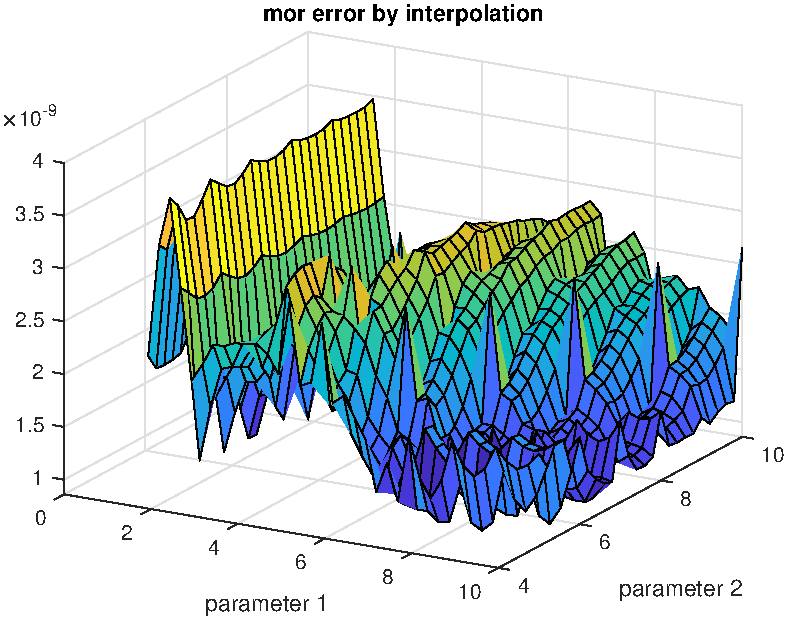
\includegraphics[width=1\textwidth]{pdfFIG/morerr_interp.pdf}\\
		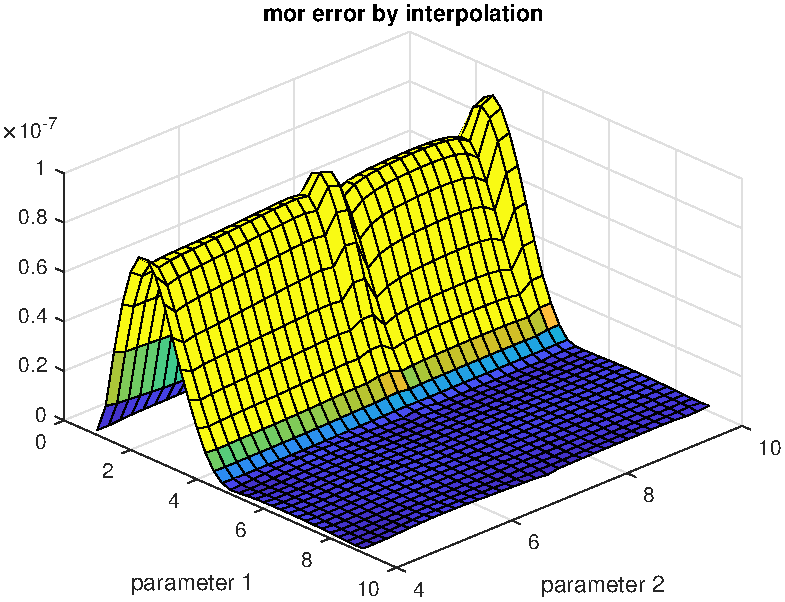
\includegraphics[width=1\textwidth]{pdfFIG/morerr_interp3.pdf}
		%\hspace*{.4\textwidth} (a)
	\end{minipage}%\hspace*{2mm}
	\begin{minipage}{.5\textwidth}
		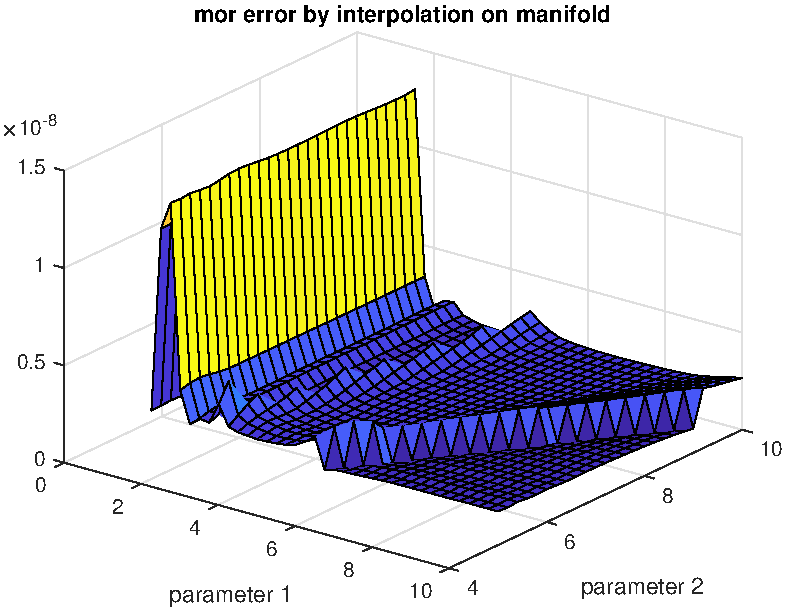
\includegraphics[width=1\textwidth]{pdfFIG/morerr_maninterp.pdf} \\
		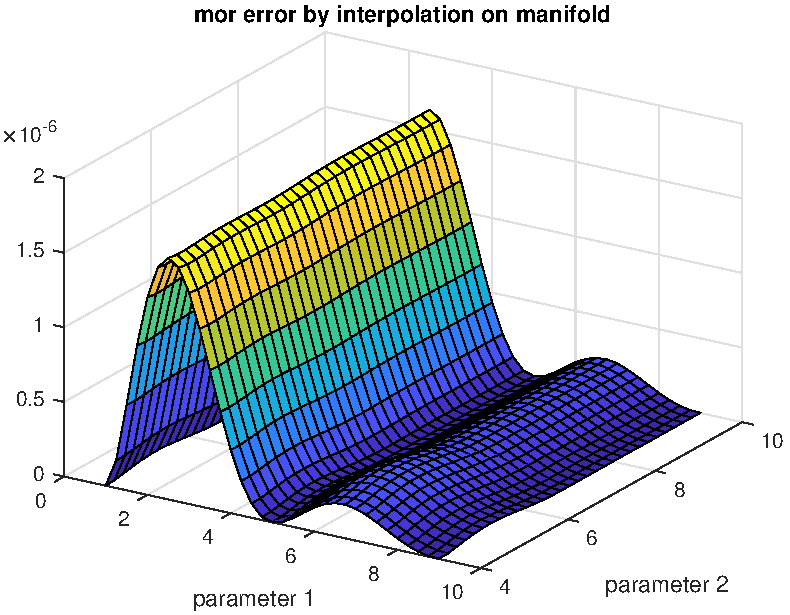
\includegraphics[width=1\textwidth]{pdfFIG/morerr_maninterp3.pdf}
		%\hspace*{.4\textwidth} (b)
	\end{minipage}
	\caption{The heat conduction model equation: errors of ROMs at test points. Data for top figures: training grid $\mu_1 = 1:1:10, \mu_2 = 5:1:10$ and test grid $\mu_1 = 1:0.25:10, \mu_2 = 5:0.2:10$; data for bottom figures: training grid $\mu_1 = 1:4:9, \mu_2 = 4:3:10$ and test grid $\mu_1 = 1:0.25:9, \mu_2 = 4:0.2:10$. The left figures present the error of the ROMs produced by the algebraic method and the right figures present that by the geometric method.}
	\label{fig:err_example1}
\end{figure}

First, we fix a uniform grid $\mu_1,\dots, \mu_q \in \mathcal{D}$ , which will be specified in the caption of error figures. At those points, we solve \eqref{eq:LyapContr} and \eqref{eq:LyapObser} using the low-rank ADI method \cite{LiW02} with a prescribed tolerance $1\mbox{e}-10$. We end up with local approximate solutions whose rank varies from 25 to 27. In order to apply the presented interpolation on manifold, we slightly truncate them to make them all of rank 25. Then, the working manifold in this case is $\mathcal{S}_+(25,1580)$. Note that for method presented in section~\ref{Sec:BT_standard interpolation}, local solutions at training points do not necessarily have the same rank.

The pre-computed solutions are then employed as data to interpolate for evaluate the two gramians which in turn are use to construct the ROM at test points. To decide the reduced order, we use the criterion that $\sigma_r(\mu)/\sigma_1(\mu) < 1\mbox{e}-8$ which varies $r$ between 12 to 15 at different test points. Finally, we plot the approximate absolute errors with respect to $\mathcal{H}_\infty$-norm as defined in \eqref{eq:errH}. For ease of reading numerical results as figures, we simply choose the set o test points as a finer grid of the training grid which will be specified later. Two situations are set and the corresponding results are showed in Figure~\ref{fig:err_example1}. It can be observed that, in the same setting, the algebraic method delivers a slightly smaller error than the geometric one. This is most probably due to the truncation step to make all the local gramians have the same rank. %To verify this, we perform another test for the algebraic method where the interpolated data are the same as those used for the geometric method. The setting is the same as the top part of Figure~\ref{fig:err_example1} and the corresponding result is showed in Figure~\ref{fig:err2_example1} left. The error is then of the same order as geometric method (Fig.~\ref{fig:err_example1} top - right).
 Moreover, the figures show that the error corresponding to small $\mu_1$ tends to be larger. This suggests that we should use more interpolation data in this area. To this end, we try an adaptively finer grid for the algebraic method and derived the result as showed in Figure~\ref{fig:err2_example1} left. Finally, to give the reader a view on the relative errors of the method, we plot the $\mathcal{H}_\infty$-norm of the full-order transfer function in Figure~\ref{fig:err2_example1} right.

\begin{figure}[th]
	\begin{minipage}{.5\textwidth}
	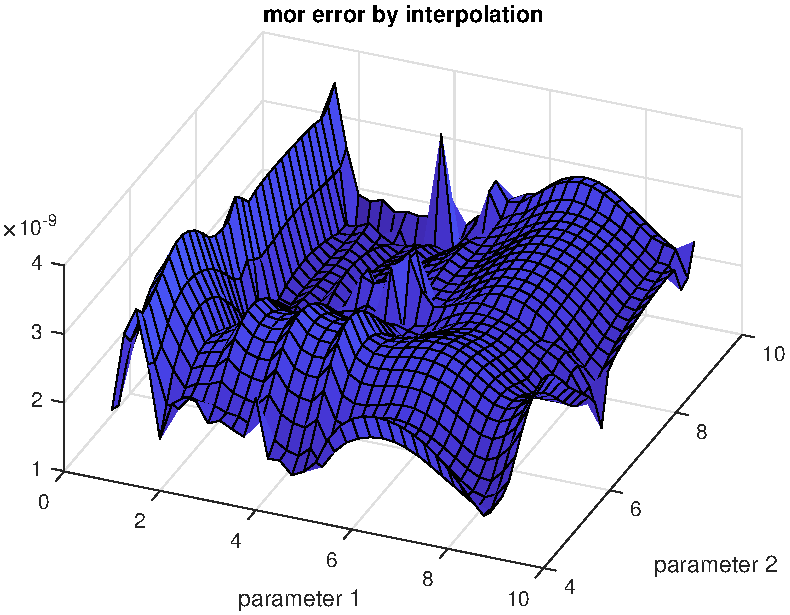
\includegraphics[width=\textwidth]{pdfFIG/morerr_interp4.pdf}\\
		%\hspace*{.4\textwidth} (a)
	\end{minipage}
	\begin{minipage}{.5\textwidth}
		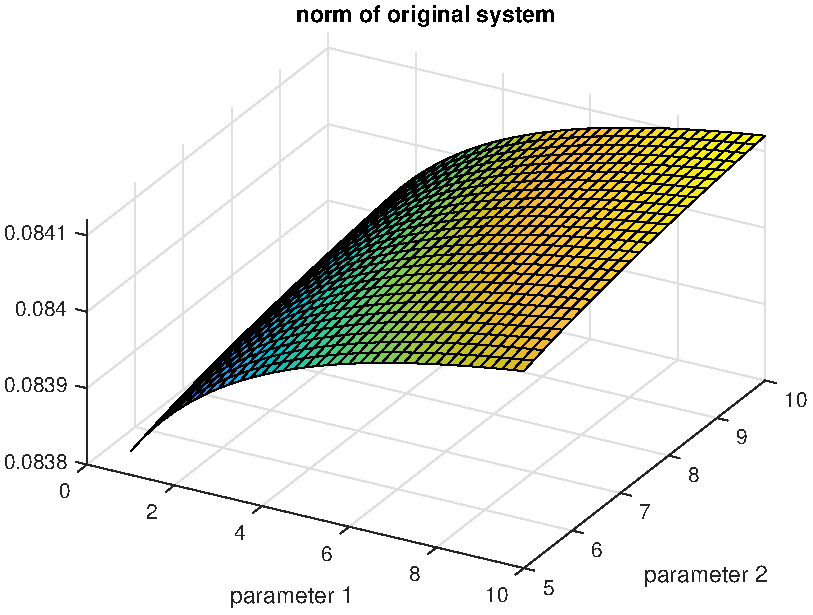
\includegraphics[width=\textwidth]{pdfFIG/nrmorig2.pdf} %\\
		%\hspace*{.4\textwidth} (b)
	\end{minipage}
	\caption{The heat conduction model equation: errors of ROMs at test points. The left figure presents the error with adaptive grid $\mu_1 = [1\ 2\ 3\ 4\ 5\ 9], \mu_2 = 4:3:10$. The right figure indicates the norm of the full-order transfer function on the parameter domain.}
	\label{fig:err2_example1}
\end{figure}

We now report the time consumed by the two proposed methods. We will use the first setting that produced the errors as showed in Figure~\ref{fig:err2_example1} top. First, solving two Lyapunov equations at 60 training points needs ..... sec. Then, interpolation of low-rank solutions of these two equations using the geometric approach at 926 test points costs .... sec. From the difference in time consumed, clearly this method can be a good candidate for quickly computing the solutions of parametric Lyapunov equations. 

\nts{I will add later!}

\nts{tried algebraic approach with compression/projection}

\subsection{An anmometer model}
In this second example, we want to verify the numerical behavior of the proposed methods when applied to fairly large problem. To this end, we consider now a model for a~thermal based flow sensor; see \cite{MoosRGKH05} and references therein. 
Simulation of this device requires solving a convection-diffusion partial differential equation of the form
\begin{equation}\label{Sec7CDPDEs}
\rho c \frac{\partial \vartheta}{\partial t} = \nabla(\kappa \nabla \vartheta)-\rho cv\nabla \vartheta +\dot{q},
\end{equation}
where $\rho$ denotes the mass density, $c$ %\in [0,1]$
 is the specific heat, $\kappa$
  %\in [1,2]$
   is the thermal conductivity, 
$v$
%\in [0.1,2]$
 is the fluid velocity, $\vartheta$ is the temperature, and $\dot q$ is the heat flow into the system 
caused by the heater. The considered model is restricted to the case $\rho = 1, c = 1, \kappa = 1$ and $v \in [0,1]$ which correseponds to the 1-parameter model. The finite element discretization of 
\eqref{Sec7CDPDEs} leads to system \eqref{eq:psys} of order $N=29008$ with the symmetric positive definite mass matrix $E(\mu) = E$ 
and the stiffness matrix $A(\mu)=A_1+vA_2$, where 
$A_1$ is symmetric negative definite, $A_2$ is non-symmetric but negative semi-definite.
The input matrix $B\in\mathbb{R}^N$ and the output matrix $C\in\mathbb{R}^{1\times N}$ are parameter-independent.
The reader is referred to \cite{morwiki_anemom} and references therein for more detailed descriptions and the numerical data.



\section{Conclusion}\label{Sec:Concl}




% BibTeX users please use one of
%\bibliographystyle{spbasic}      % basic style, author-year citations
\bibliographystyle{spmpsci}      % mathematics and physical sciences
%\bibliographystyle{spphys}       % APS-like style for physics
\bibliography{references}   % name your BibTeX data base

% Non-BibTeX users please use
%\begin{thebibliography}{}
%
% and use \bibitem to create references. Consult the Instructions
% for authors for reference list style.
%
%\bibitem{RefJ}
%% Format for Journal Reference
%Author, Article title, Journal, Volume, page numbers (year)
%% Format for books
%\bibitem{RefB}
%Author, Book title, page numbers. Publisher, place (year)
%% etc

\end{document}
% end of file template.tex

